%%%%%%%%%%%%%%%%%%%%%%%%%%%%%%%%%%%%%%%%%%%%%%%%%%%%%%%%%%%%%%%%%%%%%%%%
%                                                                      %
%     File: Thesis_Results.tex                                         %
%     Tex Master: Thesis.tex                                           %
%                                                                      %
%     Author: Andre C. Marta                                           %
%     Last modified :  4 Mar 2024                                      %
%                                                                      %
%%%%%%%%%%%%%%%%%%%%%%%%%%%%%%%%%%%%%%%%%%%%%%%%%%%%%%%%%%%%%%%%%%%%%%%%

\chapter{iQAQE Schemes and Results}
\label{chapter:Schemes_and_Results}

% Before I start mindlessly dumping things here, I should re-read everything on the logbook, so I have a better idea of what I want to say. Also, I shouldn't include all of what is said there, probably. I think I'll just write all that I want to say and, if need be, I'll cut some things in the end, once I'm re-reading the ENTIRE thing, again.

% Insert your chapter material here. - In this chapter, we should present all the many schemes that we've come up with, and the results of the numerical simulations of these schemes. We should also compare the results of the different schemes, and discuss the potential of each one. We should also mention the importance of the results and the potential applications of the schemes. This will, surely, be the largest chapter of the thesis.

% Here, I should present each realization of iQAQE, theoretically, as well as the results of the numerical simulations of each realization. I should also mention that this work is, essentially, a collection/compilation of different schemes/ideas, all inspired by the base-iQAQE algorithm, described above. As such, some schemes will appear disconnected from others, but they all serve the same purpose, ultimately. (This is how I should justify the existence of so many schemes, and the lack of a clear connection between them. Also, this is how one should look at this.)

% I might re-order these a little.


In this chapter, we present the various \acrshort{iqaqe} schemes we have developed and the results of their numerical simulations. These schemes explore different combinations of qubit numbers, list cardinalities, basis state mappings, and circuit layers. Each scheme features a unique mapping, resulting in distinct outcomes and properties. We compare these results and discuss the potential of each scheme. This chapter is essentially a collection of various ideas, all built upon the \acrshort{iqaqe} Framework described in Chapter \ref{chapter:Base Algorithm}. While some schemes may seem disconnected, they all contribute to the overall goal, justifying their inclusion.

At times, our work diverged from \acrshort{iqaqe}, leading us to explore other ideas for MaxCut algorithms. Although these ideas originated from our work on \acrshort{iqaqe}, they are distinct enough to warrant their own chapter. These will be presented in the next chapter (Chapter \ref{chapter:Exploratory_Ideas}).

From here onwards, unless explicitly stated otherwise, all \acrshort{vqa}\textcolor{gray}{s} are being tested on the following $8$-node graph, whose optimal cut is $10$ (Figure \ref{fig:8_node_graph}). This graph is one of the benchmarks used in \cite{tenecohen2023variational}, which is why we employ it here. Additionally, its small size allows for reasonably quick simulations on my personal computer, which is a significant advantage.

\begin{figure}[H]
    \centering
    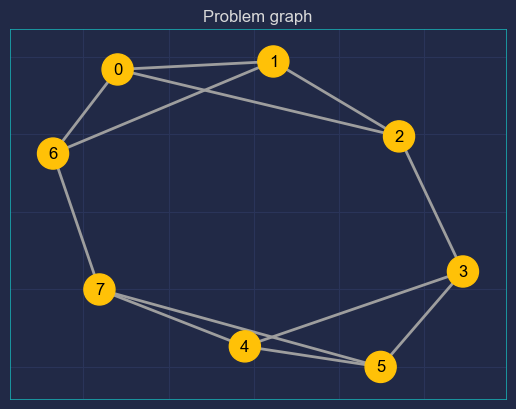
\includegraphics[width=0.55\textwidth]{Figures/Chapter_5/problem_graph.png}
    \caption{Considered $8$-node graph instance. The optimal cut ($10$) was found through
    brute-force (exhaustive search).}
    \label{fig:8_node_graph}
\end{figure}

%%%%%%%%%%%%%%%%%%%%%%%%%%%%%%%%%%%%%%%%%%%%%%%%%%%%%%%%%%%%%%%%%%%%%%%%
\section{Random iQAQE}
\label{section:Base_iQAQE}

% I think I'm going to be re-running many algorithms. This might take me some time, but I believe it is necessary.

First and foremost, we aim to understand how \acrshort{iqaqe} compares with both \acrshort{qaoa} and \acrshort{qemc}. In terms of \acrshort{iqaqe}'s implementation for this comparison, the selection of the number of qubits ($n$) and the list cardinalities ($c$) was not carefully considered. They were randomly chosen using \texttt{np.random.randint}, resulting in $n = 4$ and $c = 4$. Currently, the allocation of basis states to lists is also done randomly, without ensuring that all basis states are utilized. The goal of this initial simulation is to take a preliminary look at \acrshort{iqaqe}'s performance and understand how much the results vary between finite shot number simulations and analytical ones. (This also serves as a comparison test between the two previously mentioned Pennylane devices.) The plots below display the best-so-far average approximation ratio, derived from $10$ \acrshort{iqaqe} runs, each with different random initial parameters. The results for all three algorithms are generated using a configuration of $4$ ansatz layers and an Adam learning rate of $0.99$.

%%%%%%%%%%%%%%%%%%%%%%%%%%%%%%%%%%%%%%%%%%%%%%%%%%%%%%%%%%%%%%%%%%%%%%%%
\begin{figure}[ht!]
  \centering
  \begin{subfigure}[H]{0.495\textwidth}
      \centering
      \caption*{(a) Shots = None (Infinite)}
      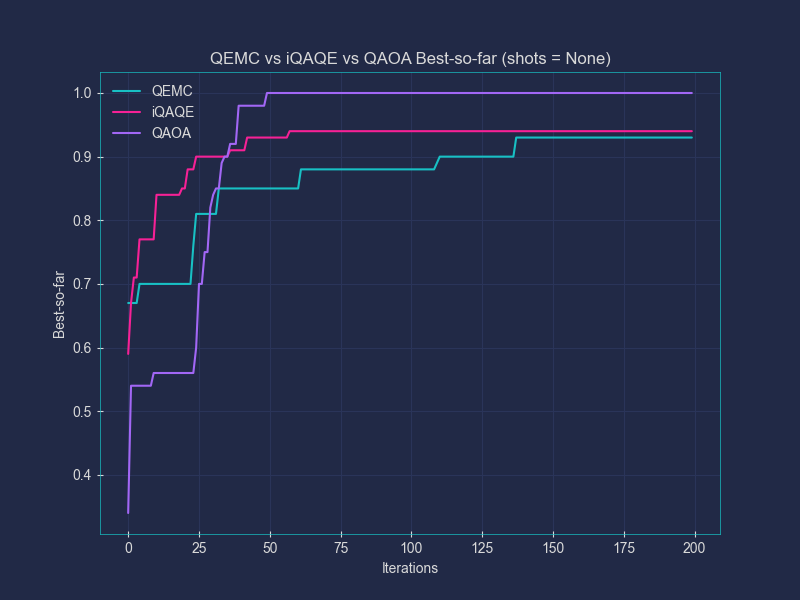
\includegraphics[width=1\textwidth]{Figures/Chapter_5/3_Comparison_shots=None.png}
      \label{fig:3_Comparison_shots=None}
  \end{subfigure}
  \hspace{-1.5em}
  \begin{subfigure}[H]{0.495\textwidth}
      \centering
      \caption*{(b) Shots = 1024}
      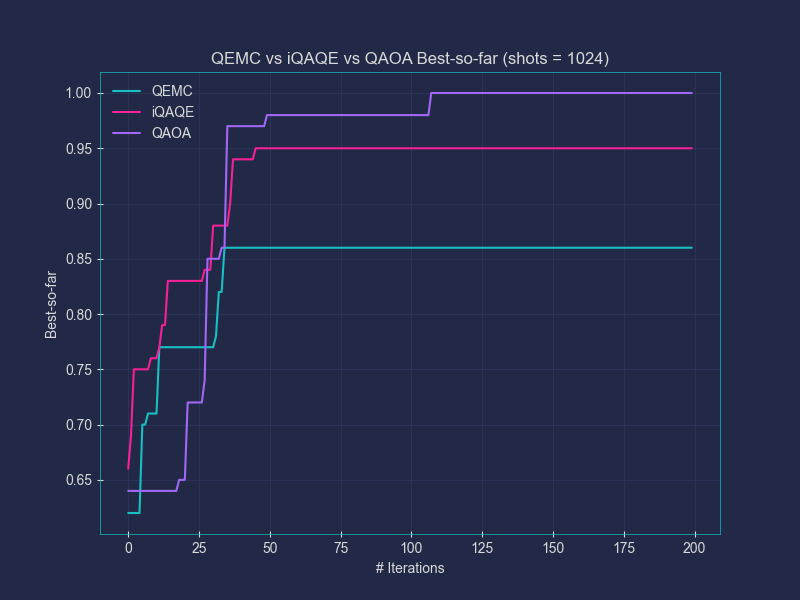
\includegraphics[width=1\textwidth]{Figures/Chapter_5/3_Comparison_shots=1024.png}
      \label{fig:3_Comparison_shots=1024}
  \end{subfigure}

  \vspace{-1.5em} % Adjust the space between the rows

  \begin{subfigure}[t]{0.495\textwidth}
      \centering
      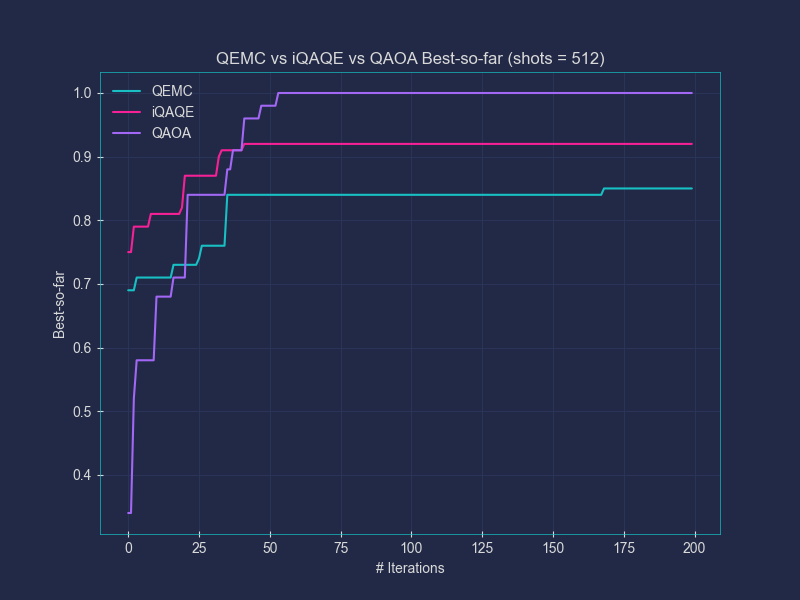
\includegraphics[width=1\textwidth]{Figures/Chapter_5/3_Comparison_shots=512.png}
      \caption*{(c) Shots = 512}
      \label{fig:3_Comparison_shots=512}
  \end{subfigure}
  \hspace{-1.5em}
  \begin{subfigure}[t]{0.495\textwidth}
      \centering
      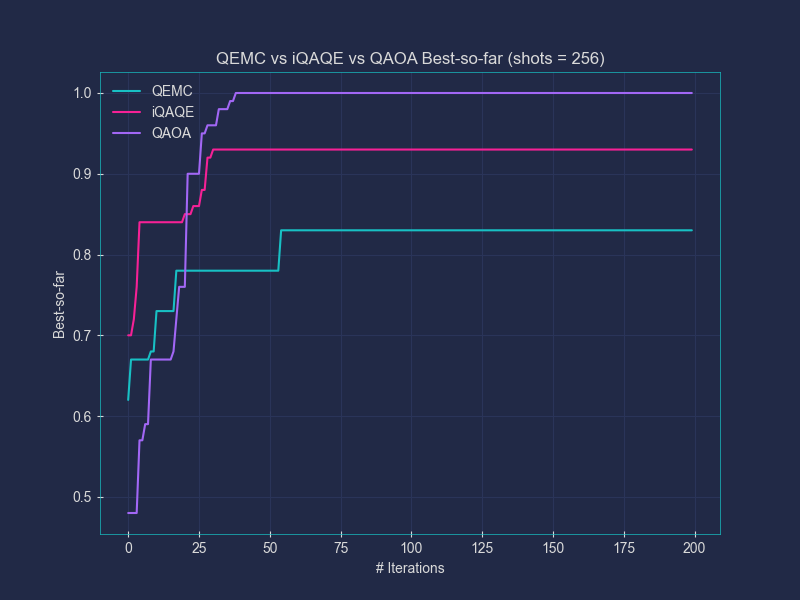
\includegraphics[width=1\textwidth]{Figures/Chapter_5/3_Comparison_shots=256.png}
      \caption*{(d) Shots = 256}
      \label{fig:3_Comparison_shots=256}
  \end{subfigure}
  
  \caption{Comparison between the $3$ \acrshort{vqa}\textcolor{gray}{s}' performances (\acrshort{qaoa}, \acrshort{qemc} and \acrshort{iqaqe}), using an infinite and finite number of shots. The best-so-far average is plotted.}
  \label{fig:3_Comparison_shots}
\end{figure}
%%%%%%%%%%%%%%%%%%%%%%%%%%%%%%%%%%%%%%%%%%%%%%%%%%%%%%%%%%%%%%%%%%%%%%%%

These plots generally align with our theoretical expectations. As \acrshort{qemc} relies heavily on a large number of shots, transitioning to a finite shot number naturally impacts the results. Surprisingly, however, \acrshort{iqaqe} seems to exhibit slightly greater resilience to this effect, despite sharing \acrshort{qemc}'s cost function and ansatz. This resilience might be attributed to the presence of multiple basis states associated with each graph node, potentially reducing the need for exhaustive sampling. If some basis states are harder to sample, the probabilities of the remaining states might adapt to compensate, as governed by the \acrshort{qemc} objective function. Nonetheless, \acrshort{qaoa} consistently outperforms both approaches, highlighting its superiority. For the same number of layers, \acrshort{qaoa}'s problem-inspired ansatz and cost function consistently yield better results. To determine if \acrshort{iqaqe} can surpass \acrshort{qaoa}'s performance, extensive testing across various combinations of parameters such as $n$, $c$, number of layers, and Adam's learning rate is necessary. This will motivate some of the grid searches we conduct later in this study. However, given the vast number of potential combinations, testing all of them is impractical. Therefore, some of the more targeted mappings/encodings explored in this work aim to constrain one or more of these variables, thereby reducing the total number of combinations for testing. Following this approach, conducting grid searches over the parameter values becomes more manageable and practical to determine the optimal settings. The subsequent sections of this chapter will detail these mapping strategies.

%%%%%%%%%%%%%%%%%%%%%%%%%%%%%%%%%%%%%%%%%%%%%%%%%%%%%%%%%%%%%%%%%%%%%%%%
\section{Polynomial Compression-type Encodings}
\label{section:Polynomial_Encodings}

At this point, driven by our earlier discussion on the nature of random-based algorithms, we begin exploring more meaningful mappings. Here, we opt to fix one or more qubits to $1$ (or $0$) while allowing the remainder to vary. The number of qubits we fix ($k$) depends on the desired order of compression. This approach not only enables the utilization of fewer qubits (if $k > 1$) but also establishes the total number of qubits to be used, simplifying subsequent grid searches over parameters. By fixing $k$ qubits, we achieve polynomial compression of order-$k$ (in the number of qubits). The total number of nodes that can be encoded in this manner is determined by $\binom{n}{k} = \frac{n!}{k!(n - k)!}$, where $n$ denotes the number of qubits. Essentially, this represents the number of ways we can select $k$ qubits from the available $n$ and set them to $1$ (or $0$), each combination encoding one graph node. Consequently, we need to ensure that $\binom{n}{k} \geq N$, where $N$ represents the number of graph nodes. This criterion guides our selection of $n$ and $k$. In practice, to determine $n$ for any $k$, we select the smallest $n$ that satisfies $\binom{n}{k} \geq N$. This yields $N = \mathcal{O}(n^k)$. Subsequently, we decide on the number of basis states to associate with each graph node, chosen from a total of $2^{n-k}$. While we could potentially utilize all $2^{n-k}$ basis states for each node (with $n-k$ free qubits), we allow for the flexibility to choose only $c \leq 2^{n-k}$. The value of $c$ requires optimization. With the mapping established, the algorithm proceeds as before, employing \acrshort{qemc}'s cost function and ansatz. Notably, we cannot use \acrshort{qaoa}'s ansatz since $n \neq N$. Due to polynomial compression, $n < N$ always, unless $k = 1$ (in which case there is no compression).






%%%%%%%%%%%%%%%%%%%%%%%%%%%%%%%%%%%%%%%%%%%%%%%%%%%%%%%%%%%%%%%%%%%%%%%%
\subsection{Basic Polynomial Compression-type iQAQE}
\label{subsection:Basic_Poly-Comp_iQAQE}


This is the simplest type of polynomial compression-based \acrshort{iqaqe} scheme. It involves fixing $k$ qubits to $1$ instead of $0$. The number of fixed qubits ($k$) is determined by the desired order of compression, as previously described. The results for $k = 2$ and $k = 3$ are shown below (Figures \ref{fig:Comparison_k2+k3_1} and \ref{fig:Comparison_k2+k3_2}). In the figures, the list cardinality is set to $4$ for both the $k = 2$ curve (\texttt{iQAQE\_k2}) and the $k = 3$ curve (\texttt{iQAQE\_k3}). Additionally, the number of layers is set to $4$ for $k = 2$ and $5$ for $k = 3$, with an Adam learning rate of $0.98$. The final curves are derived from $10$ runs of the algorithms, each with different random initial parameters. The results are compared with those of \acrshort{qaoa} and \acrshort{qemc}.

\begin{figure}[H]
  \centering
  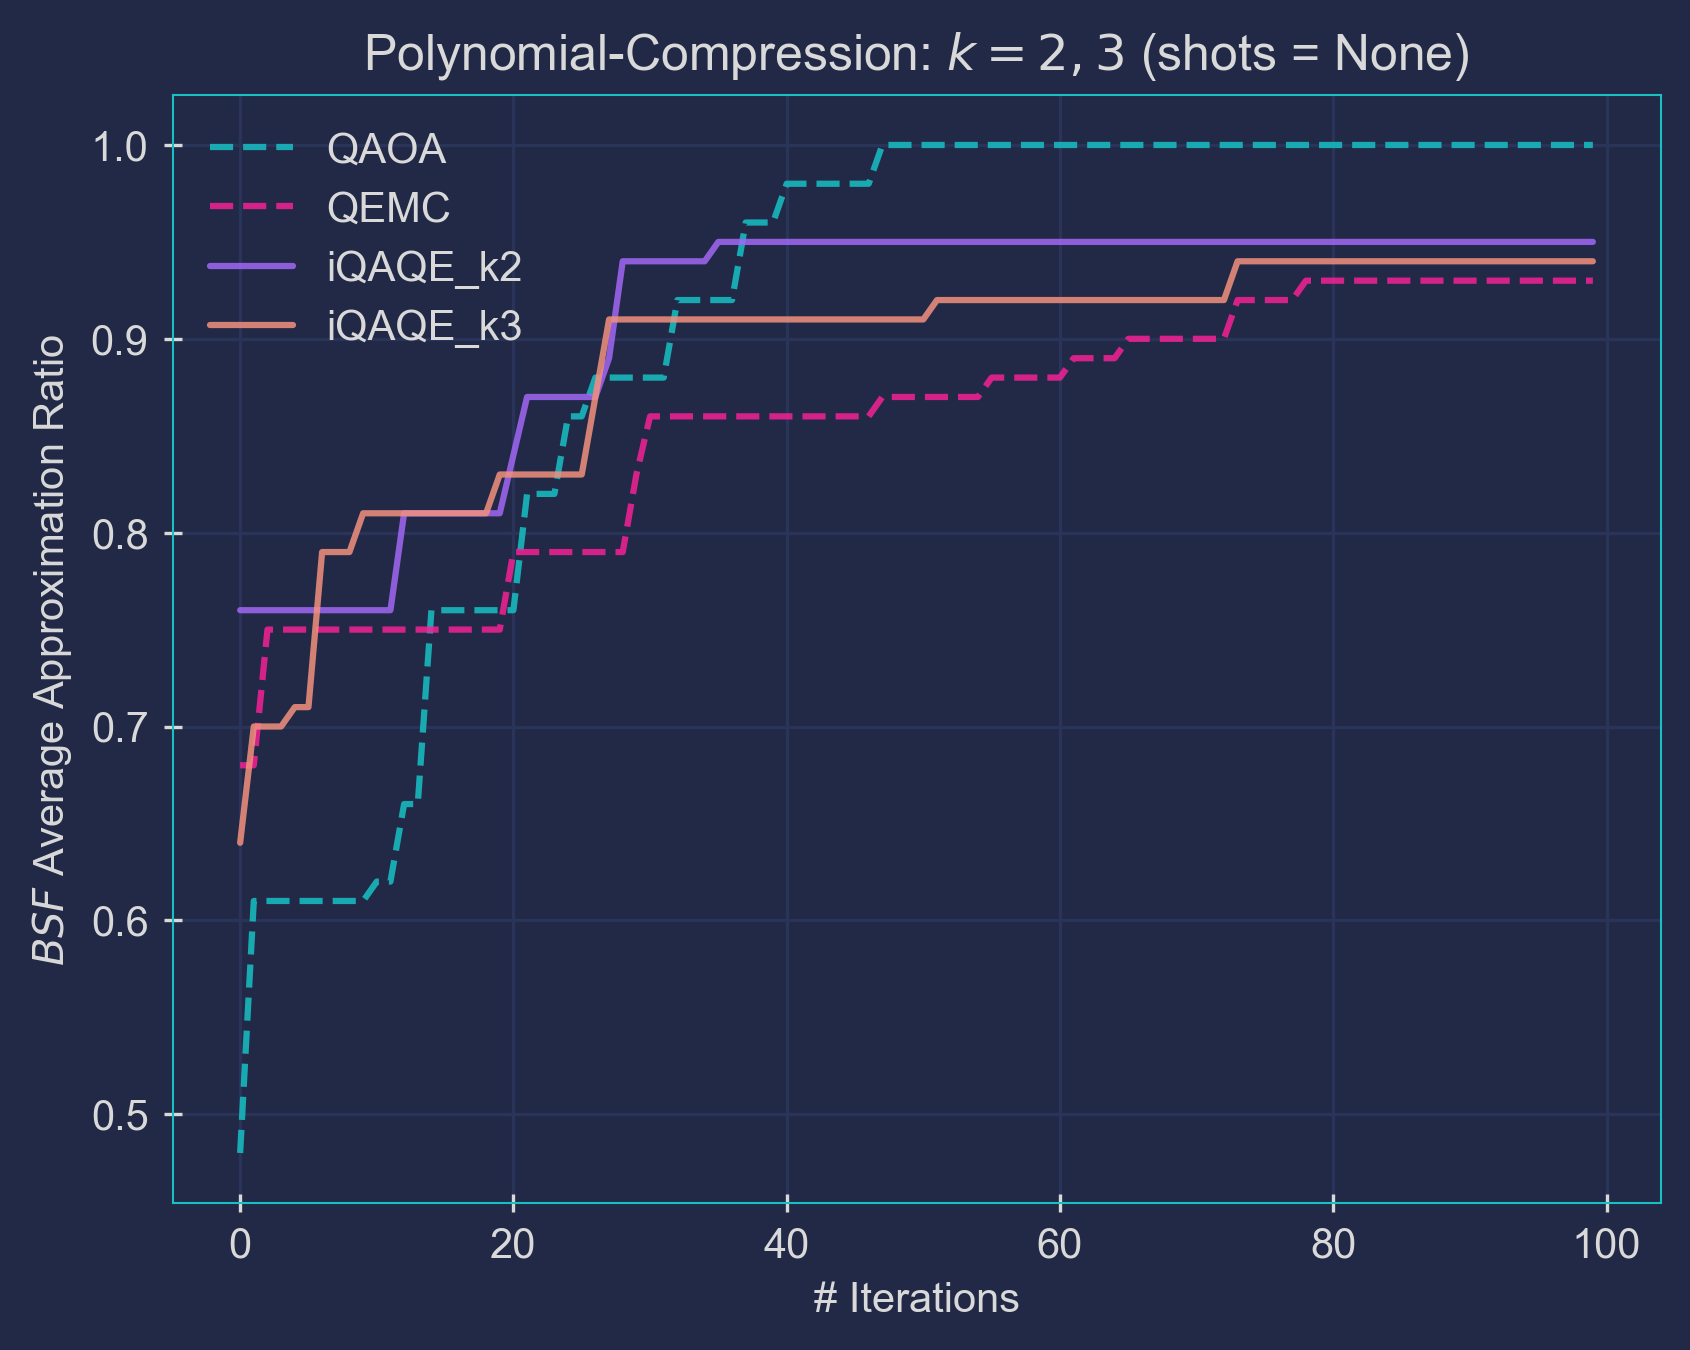
\includegraphics[width=0.70\textwidth]{Figures/Chapter_5/Polynomial_Compression_Base_k2_k3_2.png}
  \caption{\acrshort{bsf} Average Approximation Ratio \textit{vs.} iteration number for the tested \acrshort{vqa}\textcolor{gray}{s}: \acrshort{qaoa}, \acrshort{qemc}, and \acrshort{iqaqe}, using the aforementioned polynomial compression scheme. The number of layers considered were $4$ for $k = 2$ and $5$ for $k = 3$}
  \label{fig:Comparison_k2+k3_1}
\end{figure}

\begin{figure}[H]
  \centering
  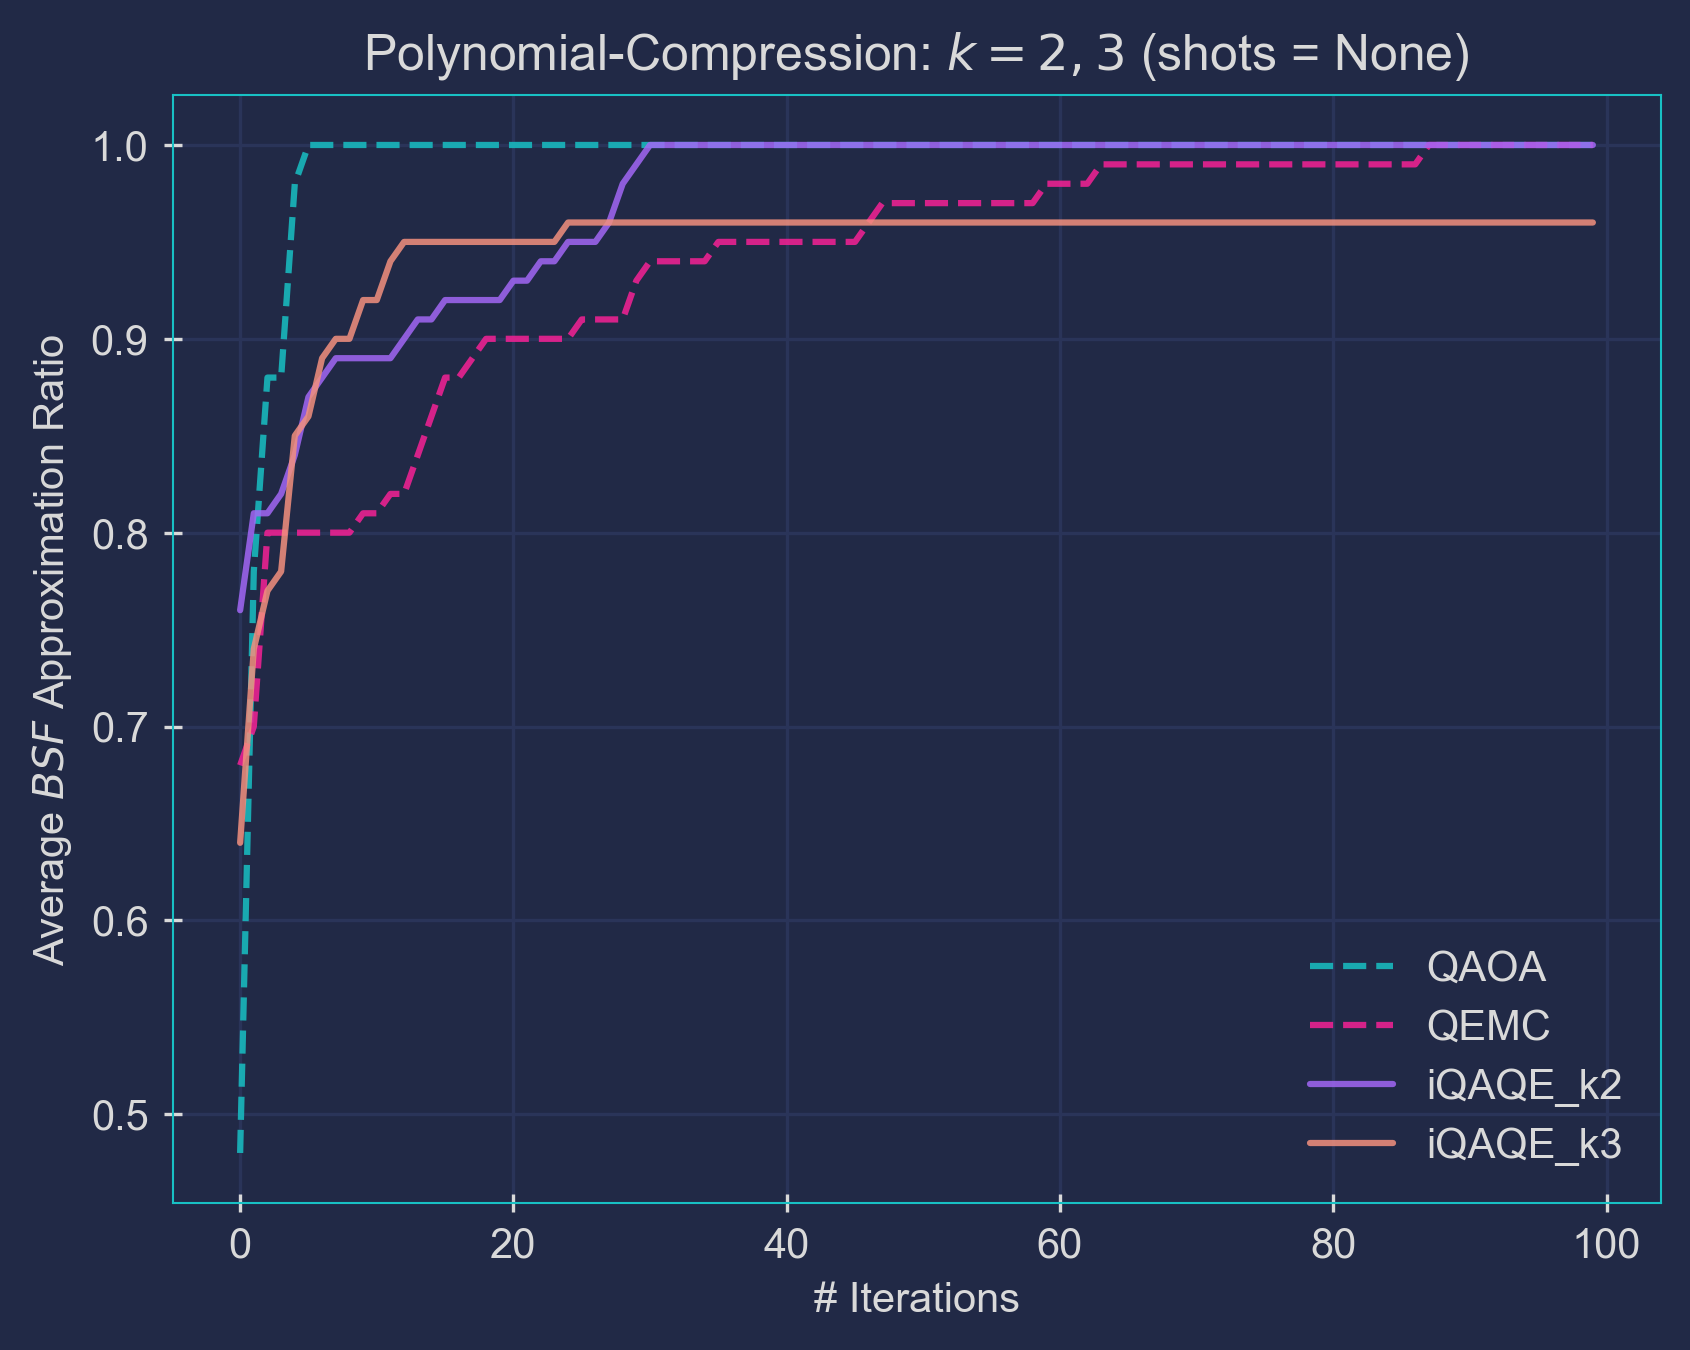
\includegraphics[width=0.70\textwidth]{Figures/Chapter_5/Polynomial_Compression_Base_k2_k3_1.png}
  \caption{Average \acrshort{bsf} Approximation Ratio \textit{vs.} iteration number for the tested \acrshort{vqa}\textcolor{gray}{s}: \acrshort{qaoa}, \acrshort{qemc}, and \acrshort{iqaqe}, using the aforementioned polynomial compression scheme. The number of layers considered were $4$ for $k = 2$ and $5$ for $k = 3$}
  \label{fig:Comparison_k2+k3_2}
\end{figure}



Notice the difference between the two figures. In the first figure, we average the curves first and then apply the \acrshort{bsf} transformation. In the second figure, we reverse the process: first applying the \acrshort{bsf} transformation to each curve and then averaging the transformed curves. The results are quite different, as illustrated. This indicates that both \acrshort{qemc} and \acrshort{iqaqe} are generally more susceptible to outliers due to particularly unlucky initial parameterizations. This is an important consideration when interpreting the forthcoming results. Often, we will choose to discard the \acrshort{bsf} average in favor of the average \acrshort{bsf}. Nonetheless, both approaches are valuable for evaluating the algorithms' properties. Additionally, in some instances, we will simply use the average. Each case will be clearly specified.

Anyways, the primary aim of this study was to assess whether different types of mappings, like the one explored here, offer advantages compared to the random case. The results in Figures \ref{fig:Comparison_k2+k3_1} and \ref{fig:Comparison_k2+k3_2} indicate that this may be the case. At the very least, they suggest that there is potential in exploring these ideas further. For example, \texttt{iQAQE\_k2} achieves a perfect approximation ratio, although it requires more iterations than \acrshort{qaoa}. Nevertheless, our method surpasses \acrshort{qemc} for $k = 2$. The results for $k = 3$ are less encouraging. However, both mappings use fewer qubits ($n = 5$) than \acrshort{qaoa} ($n = 8$), which is beneficial for implementation on practical (\acrshort{nisq}) quantum computers. The next step is to conduct grid searches over the parameters for this specific graph instance to determine if we can consistently achieve better performance than \acrshort{qaoa}. This might provide further insights into the underlying principles of the algorithm's performance.

% k=2:
\begin{figure*}[ht!]
  \centering
  \begin{subfigure}[b]{0.325\textwidth}
      \centering
      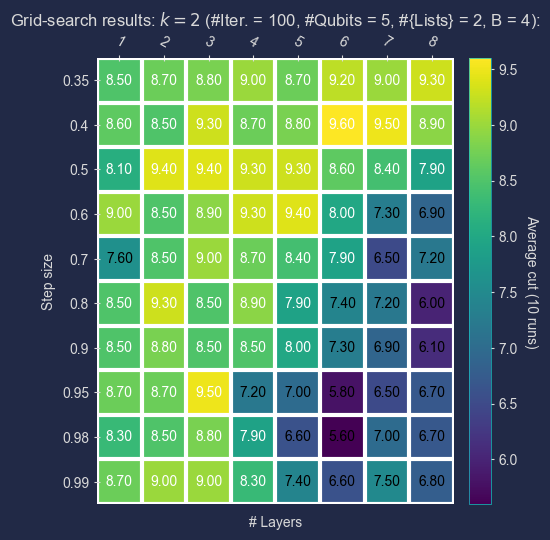
\includegraphics[width=1\textwidth]{Figures/Chapter_5/k=2(Grid_Search)/iQAQE_k2_Grid_Search_step_size_n_layers_c=2.png}
      \caption{\texttt{k = 2; c = 2}}
      \label{fig:k=2;c=2}
  \end{subfigure}
  \hfill
  \begin{subfigure}[b]{0.325\textwidth}
      \centering
      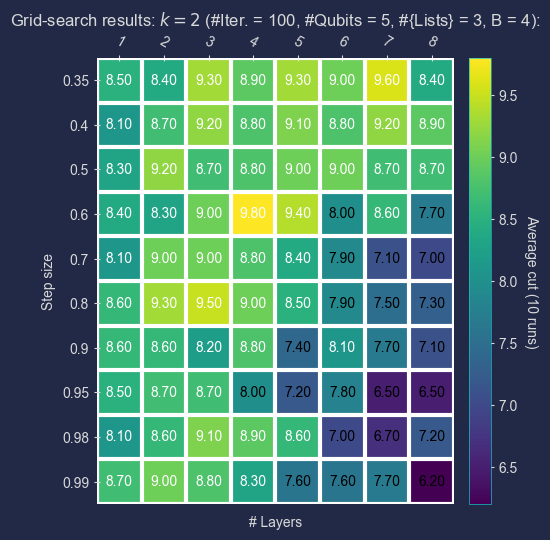
\includegraphics[width=1\textwidth]{Figures/Chapter_5/k=2(Grid_Search)/iQAQE_k2_Grid_Search_step_size_n_layers_c=3.png}
      \caption{\texttt{k = 2; c = 3}}
      \label{fig:k=2;c=3}
  \end{subfigure}
  \hfill
      \begin{subfigure}[b]{0.325\textwidth}
      \centering
      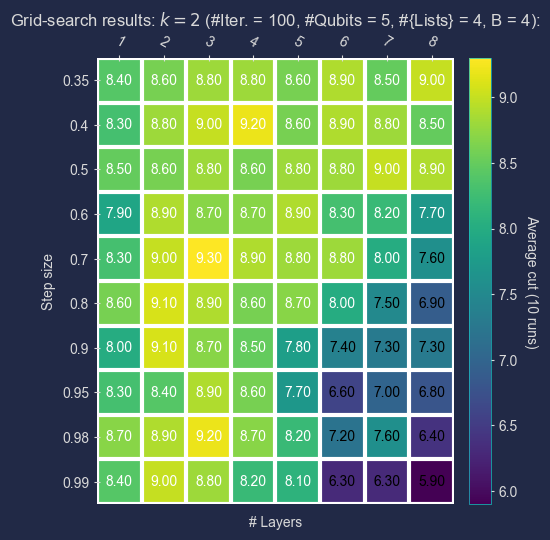
\includegraphics[width=1\textwidth]{Figures/Chapter_5/k=2(Grid_Search)/iQAQE_k2_Grid_Search_step_size_n_layers_c=4.png}
      \caption{\texttt{k = 2; c = 4}}
      \label{fig:k=2;c=4}
  \end{subfigure}
  \bigskip
  \begin{subfigure}[b]{0.325\textwidth}
      \addtocounter{subfigure}{3} % Added <<
      \centering
      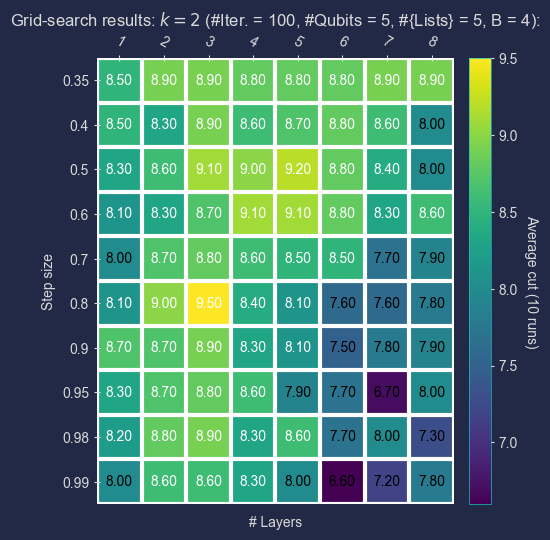
\includegraphics[width=1\textwidth]{Figures/Chapter_5/k=2(Grid_Search)/iQAQE_k2_Grid_Search_step_size_n_layers_c=5.png}
      \caption{\texttt{k = 2; c = 5}}
      \label{fig:k=2;c=5}
  \end{subfigure}
  \hfill
  \begin{subfigure}[b]{0.325\textwidth}
      \centering
      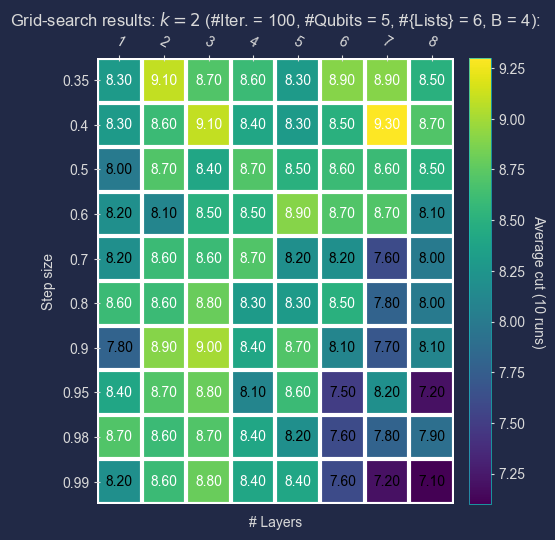
\includegraphics[width=1\textwidth]{Figures/Chapter_5/k=2(Grid_Search)/iQAQE_k2_Grid_Search_step_size_n_layers_c=6.png}
      \caption{\texttt{k = 2; c = 6}}
      \label{fig:k=2;c=6}
  \end{subfigure}
  \hfill
  \begin{subfigure}[b]{0.325\textwidth}
      \centering
      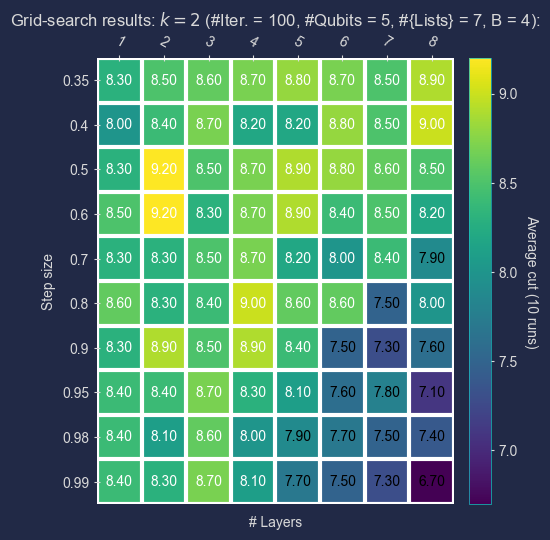
\includegraphics[width=1\textwidth]{Figures/Chapter_5/k=2(Grid_Search)/iQAQE_k2_Grid_Search_step_size_n_layers_c=7.png}
      \caption{\texttt{k = 2; c = 7}}
      \label{fig:k=2;c=7}
  \end{subfigure}
  \caption{Basic Polynomial Compression-type \acrshort{iqaqe} – Grid search, using $k=2$. All the simulations were done using an infinite number of shots (\texttt{shots = None}), and each value consists of the average of $10$ \acrshort{iqaqe} instances, using different random initial parameters.}
  \label{fig:k=2}
\end{figure*}

% k=3:
\begin{figure*}[ht!]
  \centering
  \begin{subfigure}[b]{0.475\textwidth}
      \centering
      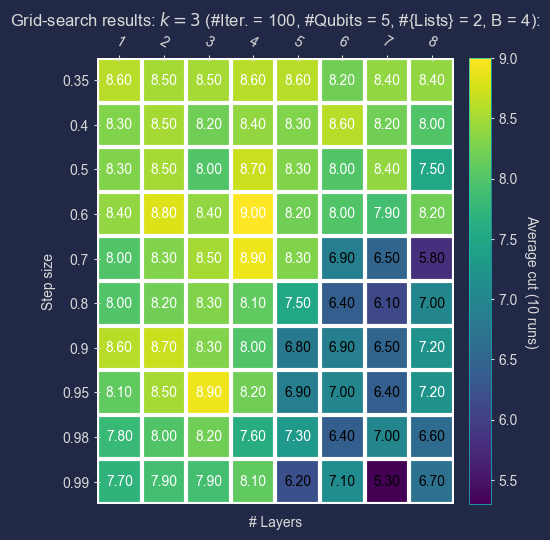
\includegraphics[width=1\textwidth]{Figures/Chapter_5/k=3(Grid_search)/iQAQE_k3_Grid_Search_step_size_n_layers_c=2.png}
      \caption{\texttt{k = 3; c = 2}}
      \label{fig:k=3;c=2}
  \end{subfigure}
  \hfill
  \begin{subfigure}[b]{0.475\textwidth}
      \centering
      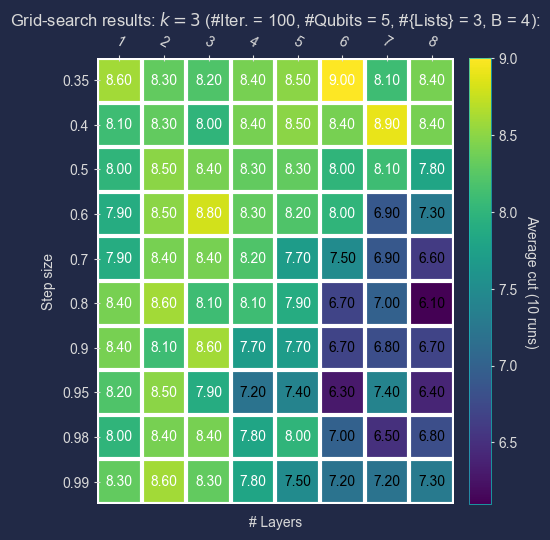
\includegraphics[width=1\textwidth]{Figures/Chapter_5/k=3(Grid_search)/iQAQE_k3_Grid_Search_step_size_n_layers_c=3.png}
      \caption{\texttt{k = 3; c = 3}}
      \label{fig:k=3;c=3}
  \end{subfigure}
  \caption{Basic Polynomial Compression-type \acrshort{iqaqe} – Grid search, using $k=3$. All the simulations were done using an infinite number of shots (\texttt{shots = None}), and each value consists of the average of $10$ \acrshort{iqaqe} instances, using different random initial parameters.}
  \label{fig:k=3}
\end{figure*}

The results of the grid searches conducted for $k=2$ and $k=3$ are present in Figures \ref{fig:k=2} and \ref{fig:k=3}. Various values were explored for the parameters: \texttt{step\_size\_list = [0.35, 0.4, 0.5, 0.6, 0.7, 0.8, 0.9, 0.95, 0.98, 0.99]}, \texttt{n\_layers} ranging from $1$ to $8$, and \texttt{c} varying from $2$ to $(2^{\texttt{n - k}} - 1)$, for $k=2, 3$, where \texttt{n\_layers} and \texttt{c} are integers. Notably, all simulations for the grid searches were executed with an infinite number of shots (\texttt{shots = None}). Additionally, this time, we utilized the average curve (from $10$ instances) instead of the average best-so-far curve. This choice was made to evaluate the overall performance of the algorithm rather than focusing solely on the best-performing instances. Each run continued until convergence (\texttt{abs\_tol <= 1e-5}) or \texttt{max\_iter = 1000} was reached, followed by recording the final partition's cut. The objective was to identify any discernible patterns in the grid search to enhance the scheme's performance. However, no apparent pattern emerged, highlighting a recurring challenge in this work: the abundance of hyperparameters makes it challenging to optimize results through straightforward means. Later, we will explore employing a more intricate machine learning scheme to address this challenge. For now, we proceed with a different approach.

% Then, it's grid-search(es).
% After that, recovery of the QAOA limit.
% Finally, other values of $k$. Actually, what I have now should be under this subsubsection, instead of the one above. I'll fix this, tomorrow.

% Then, I can quickly go through correlation-based iQAQE and fixed-parity iQAQE. I'll leave this for tomorrow, as well.

% Afterwards, Extended-QEMC, and all the other surrounding topics.





%%%%%%%%%%%%%%%%%%%%%%%%%%%%%%%%%%%%%%%%%%%%%%%%%%%%%%%%%%%%%%%%%%%%%%%%
\subsubsection*{Recovering the QAOA limit ($k = 1$)}
\label{subsubsection:QAOA-Limit_iQAQE}


Next, we tested whether we could recover the \acrshort{qaoa} limit using \acrshort{iqaqe}'s algorithm with what we call the \acrshort{qaoa} mapping for this scheme. This mapping involves using the same number of qubits as there are nodes (as in standard \acrshort{qaoa}) and assigning $2^{n-1}$ basis states to each graph node. For each graph node, a different qubit is fixed to $1$, while the remaining $n - 1$ qubits are free to vary, resulting in $2^{n-1}$ basis states per node. The rest of the algorithm remains unchanged, employing \acrshort{qemc}'s ansatz and cost function. The nodes' probabilities are derived from the normalized sum of the probabilities of their associated basis states. This approach was motivated by our desire to better understand \acrshort{iqaqe}'s properties and behavior. Previously, we observed (Figure \ref{fig:3_Comparison_shots}) that \acrshort{iqaqe}'s performance seemed to fall between that of \acrshort{qaoa} and \acrshort{qemc}, which is intuitive, as it is designed as an interpolation between the two. To further test this behavior, we used \acrshort{qaoa}'s mapping to see how closely we could approach \acrshort{qaoa}'s performance levels, which have been the best so far. The following results were obtained, focusing only on analytical simulations (i.e., infinite shots) – We employ the average curve obtained from $10$ runs, as we did in the previous grid search:

\begin{figure}[H]
  \centering
  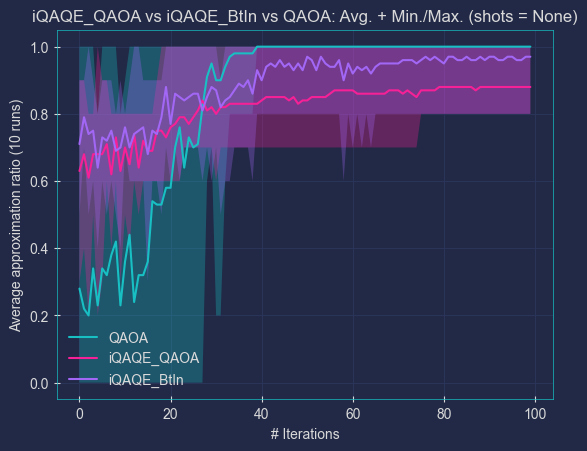
\includegraphics[width=0.70\textwidth]{Figures/Chapter_5/iQAQE_QAOA.png}
  \caption{Average approximation ratio ($\pm \sigma$) $vs$ iteration number, for the three tested \acrshort{vqa}\textcolor{gray}{s}: \texttt{QAOA}, \texttt{iQAQE\_QAOA} (as described above) and \texttt{iQAQE\_BtIn}. The latter stands for \acrshort{iqaqe}, with better initialization. This corresponds to the same mapping as the one in Figure \ref{fig:3_Comparison_shots}.}
  \label{fig:iQAQE_QAOA}
\end{figure}

This realization led us to understand that we cannot expect to replicate \acrshort{qaoa}'s outstanding performance on this graph simply by using a \acrshort{qaoa}-type encoding. After all, we are still relying on \acrshort{qemc}'s cost function and ansatz, so this outcome is not entirely surprising. Moreover, to add to the challenge, we found that \texttt{iQAQE\_QAOA}'s performance can even be surpassed by another random, non-specific mapping, highlighting how far we are from achieving \acrshort{qaoa}-like results.

In an effort to bridge this gap, we attempted to integrate \acrshort{qaoa}'s ansatz into the scheme, alongside the \acrshort{qaoa}-type encoding. However, after extensive testing, we realized this approach is not feasible. Here's why: using both elements together with the node probability encoding (as a normalized sum of their associated basis states' probabilities) causes the \acrshort{qemc} cost function to become independent of the ansatz's parameters\footnote{To verify this, we performed analytical calculations for a simple toy model: a graph with two nodes connected by a single edge. The results generalize to larger graphs.}. This means we cannot proceed with training, rendering the scheme ineffective. Thus, implementing this approach in its current form is not possible. For it to be successful, other aspects would need to change, such as the cost function or the method of deriving node probabilities from basis states' probabilities, which is the main issue here.









%%%%%%%%%%%%%%%%%%%%%%%%%%%%%%%%%%%%%%%%%%%%%%%%%%%%%%%%%%%%%%%%%%%%%%%%
% \subsection{Parity-like QAOA}
% \label{subsection:Parity_QAOA}

% Parity-like QAOA schemes and their results.

% % Send this to Chapter 6, instead.





%%%%%%%%%%%%%%%%%%%%%%%%%%%%%%%%%%%%%%%%%%%%%%%%%%%%%%%%%%%%%%%%%%%%%%%%
\subsection{Correlation-based iQAQE}
\label{subsection:Correlation_iQAQE}

This scheme closely resembles what was previously discussed in subsection \ref{subsection:Basic_Poly-Comp_iQAQE}. The key distinction lies in the inclusion of the possibility for both $0$'s and $1$'s to be fixed. Consequently, the scheme aims to identify correlations among the different qubits, wherein "correlations" denote identical colors. In other words, the constructed lists regard the $k$ fixed qubits as positively correlated, meaning they are either all set to $1$ or all set to $0$. This approach was inspired by the notion that by identifying correlations between nodes, it becomes feasible to color the entire graph as long as one node is initially colored. Although seeking correlations between qubits, as done here, differs from seeking correlations between nodes, we anticipated that it might yield promising results to some extent. In this scenario, the color of each node is determined by the probability that its $k$ associated qubits are all positively correlated.

To delve deeper into the properties and characteristics of this scheme, we conducted a thorough formal analysis, exploring its limits by considering scenarios where $k$ ranges from $1$ to $n$ qubits, covering the entire spectrum. Our primary objective was to ascertain if we could formulate this correlation-based \acrshort{iqaqe} scheme in a manner that truly interpolates between \acrshort{qaoa} and \acrshort{qemc}. We aimed to determine if we could retrieve both algorithms by adjusting the parameters accordingly. However, with this correlation-based scheme, we not only cannot recover \acrshort{qaoa}, but we also fail to retrieve \acrshort{qemc}. Thus, this does not represent an interpolation between the two algorithms.

Likewise, earlier, we loosely referred to the \acrshort{iqaqe} Framework as an interpolation. However, upon closer scrutiny, this characterization seems inaccurate. While it is possible to recover the \acrshort{qemc} limit\footnote{Simply utilize the appropriate number of qubits and select one unique basis state for each node.}, the same cannot be said for \acrshort{qaoa}, as we have observed before.

Additionally, we provide the results of numerical simulations applied to the standard $8$-node graph.

\begin{figure}[H]
  \centering
  \begin{subfigure}[t]{0.495\textwidth}
      \centering
      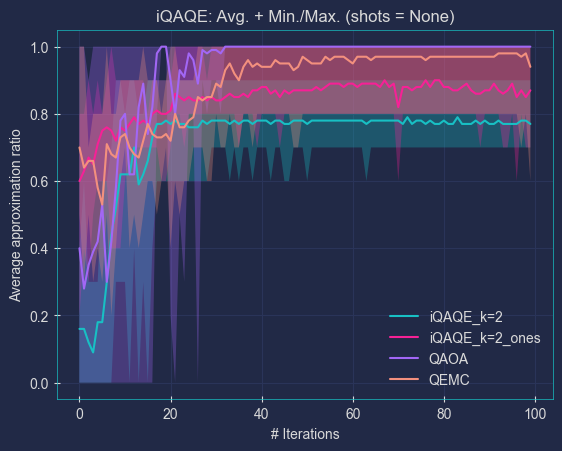
\includegraphics[width=1\textwidth]{Figures/Chapter_5/Correlation-based/k=2(Reg.+Ones).png}
      \caption{\raggedright Comparison of Correlation-based \acrshort{iqaqe} for $k=2$ with results from \acrshort{qaoa}, \acrshort{qemc}, and the previous Basic Polynomial Compression-type iQAQE\footnotemark{} (\texttt{iQAQE\_k=2\_ones}).}
      \label{fig:Correlation/k=2}
  \end{subfigure}
  \hfill
  \begin{subfigure}[t]{0.495\textwidth}
      \centering
      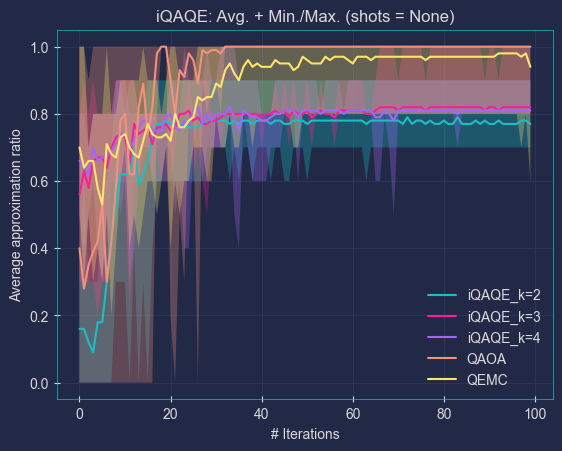
\includegraphics[width=1\textwidth]{Figures/Chapter_5/Correlation-based/k=2_3_4.png}
      \caption{Comparison of Correlation-based \acrshort{iqaqe} results for $k=2, 3$, and $4$ with outcomes from \acrshort{qaoa} and \acrshort{qemc}.}
      \label{fig:Correlation/k=2,3,4}
  \end{subfigure}
  \caption{Correlation-based polynomial-type compression scheme ($k=2, 3$ and $4$): numerical simulations for the usual $8$-node graph.}
  \label{fig:Correlation-based}
\end{figure}

\footnotetext[\value{footnote}]{This refers to the scenario where only $1$'s are fixed, not $0$'s.}

\clearpage

\begin{figure}[H]
  \centering
  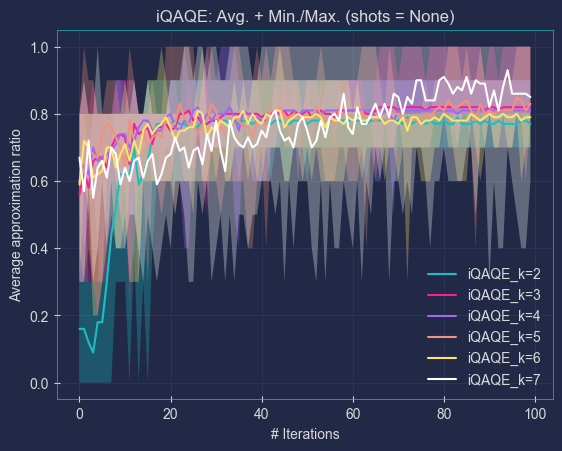
\includegraphics[width=\textwidth]{Figures/Chapter_5/Correlation-based/All_k's.png}
  \caption{Correlation-based polynomial-type compression scheme ($k = 2, 3, 4, 5, 6$ and $7$): numerical simulations for the usual $8$-node graph.}
  \label{fig:All_k's}
\end{figure}

Note that we once again use the average approximation ratio from $10$ runs, each with different random initial parameters. Additionally, we plot the average, with the shaded region representing the maximum and minimum obtained approximation ratios. Performance-wise, this scheme does not fare well. It is significantly outperformed by \acrshort{qaoa}, \acrshort{qemc}, and the basic polynomial compression-type \acrshort{iqaqe}. We also compared the results for all possible values of $k$ (Figure \ref{fig:All_k's}). It turns out that the specific value of $k$ is not very meaningful, as performance is quite similar across all values.

The underperformance is likely due to our doubling the number of basis states in each sublist. This encoding results in each pair of sublists having a $50\%$ overlap, similar to the Basic Polynomial Compression-type \acrshort{iqaqe}. However, with twice\footnote{Either $0$'s or $1$'s can be fixed.} the number of basis states this time, the number of overlapping basis states is significantly higher. This increase means that more states are shared by multiple nodes. When the overlap is too large, it becomes more challenging to adjust the color of one node without affecting the others. We believe this to be the main reason for the underperformance. We will be mindful of this in the design of future schemes.

% One of these schemes allowed to easily recover QEMC in one of its limits. Try to figure out what that was.

% Analytical analysis: do I even want to include this here? It didn't really amount to much, in the end... I'll have to think about this.





%%%%%%%%%%%%%%%%%%%%%%%%%%%%%%%%%%%%%%%%%%%%%%%%%%%%%%%%%%%%%%%%%%%%%%%%
\subsection{Fixed-Parity iQAQE}
\label{subsection:Fixed-Parity_iQAQE}

% Mention that this is a 'heuristic'. It's not a strict rule, but it's a good guideline.

In this section, we present another heuristic method for mapping the basis states to the nodes. Although it is similar to the previous one, this time we \textbf{fixed the parity of the selected $k$ qubits to be even}. Parity is determined by the number of 1's: if the count is even, the parity is even; otherwise, it is odd. For instance, for $k=3$ (with \texttt{n\_qubits = 5}), the lists would take the form: (Keep in mind that we are using an $8$-node graph.)

% Remeber that 'k=2' is the same as the previous correlation-based! Mention this in the text!

\begin{multicols}{2}
  \begin{enumerate}
    \item $\left\{\ket{000\text{xx}}, \ket{011\text{xx}}, \ket{101\text{xx}}, \ket{110\text{xx}}\right\}$;
    \item $\left\{\ket{00\text{xx}0}, \ket{01\text{xx}1}, \ket{10\text{xx}1}, \ket{11\text{xx}0}\right\}$;
    \item $\left\{\ket{0\text{xx}00}, \ket{0\text{xx}11}, \ket{1\text{xx}01}, \ket{1\text{xx}10}\right\}$;
    \item $\left\{\ket{\text{xx}000}, \ket{\text{xx}011}, \ket{\text{xx}101}, \ket{\text{xx}110}\right\}$;
    \item $\left\{\ket{\text{x}0\text{x}00}, \ket{\text{x}0\text{x}11}, \ket{\text{x}1\text{x}01}, \ket{\text{x}1\text{x}10}\right\}$;
    \item $\left\{\ket{\text{x}00\text{x}0}, \ket{\text{x}01\text{x}1}, \ket{\text{x}10\text{x}1}, \ket{\text{x}11\text{x}0}\right\}$;
    \item $\left\{\ket{\text{x}000\text{x}}, \ket{\text{x}011\text{x}}, \ket{\text{x}101\text{x}}, \ket{\text{x}110\text{x}}\right\}$;
    \item $\left\{\ket{0\text{x}0\text{x}0}, \ket{0\text{x}1\text{x}1}, \ket{1\text{x}0\text{x}1}, \ket{1\text{x}1\text{x}0}\right\}$.
  \end{enumerate}
\end{multicols}
\noindent Once again, numerical simulations were performed, and the obtained results are presented below (Figure \ref{fig:Fixed-parity}). Although the performance is still not quite on par with \acrshort{qaoa}, it is significantly better than in the previously considered scenario. Note that the case where $k=2$ corresponds to the previous correlation-based scheme. For $k=2$, requiring the pair to be even is equivalent to requiring them to be the same (either both $0$ or both $1$), which explains the similarity in results. This similarity is apparent in the less favorable outcomes shown for $k=2$ in Figure \ref{fig:Fixed-parity}, which qualitatively match those in Figures \ref{fig:Correlation-based} and \ref{fig:All_k's}. However, when we allow for $k>2$, the performance improves significantly, likely due to the reduced overlap between the basis states associated with different nodes.

A keen observer might notice that this scheme's results also allow for generating the MaxCut partition, as shown by the shaded pink region in Figure \ref{fig:Fixed-parity/k=2,3,4} for $k=3$. These shaded regions depict the maximum and minimum cuts achieved out of the $10$ runs. This reveals that, despite the greater variability and lower average performance than \acrshort{qaoa}, the algorithm can achieve the MaxCut partition in some runs. In practice, this is crucial. When running the algorithm $10$ times, our main interest is in the best outcome. This highlights the potential of this heuristic scheme.

\begin{figure}[hb!]
  \centering
  \begin{subfigure}[t]{0.495\textwidth}
      \centering
      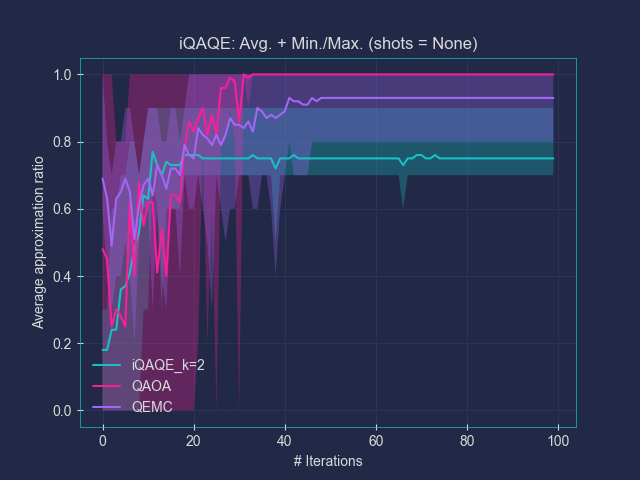
\includegraphics[width=1\textwidth]{Figures/Chapter_5/Fixed-parity/k=2(8-node).png}
      \caption{Fixed-parity \acrshort{iqaqe} for $k=2$ compared with the results from \acrshort{qaoa} and \acrshort{qemc} ($8$-node graph).}
      \label{fig:Fixed-parity/k=2}
  \end{subfigure}
  \hfill
  \begin{subfigure}[t]{0.495\textwidth}
      \centering
      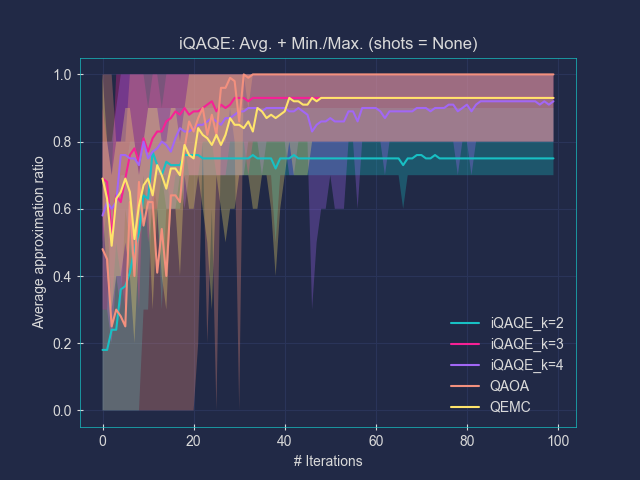
\includegraphics[width=1\textwidth]{Figures/Chapter_5/Fixed-parity/k=2_3_4(8-node).png}
      \caption{Fixed-parity \acrshort{iqaqe} for $k=2, 3$, and $4$ compared with the results from \acrshort{qaoa} and \acrshort{qemc} ($8$-node graph).}
      \label{fig:Fixed-parity/k=2,3,4}
  \end{subfigure}
\end{figure}

\clearpage

\begin{figure}[ht!]
  \addtocounter{figure}{-1} % Added <<
  \centering
  \begin{subfigure}[b]{1\textwidth}
      \addtocounter{subfigure}{2} % Added <<
      \centering
      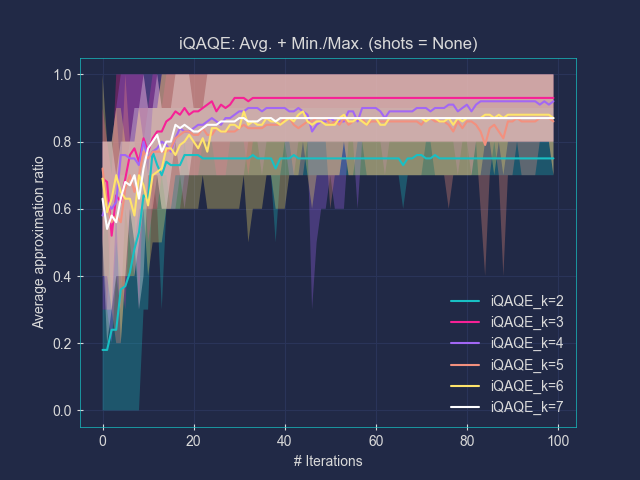
\includegraphics[width=1\textwidth]{Figures/Chapter_5/Fixed-parity/All_k's(8-node).png}
      \caption{Fixed-parity \acrshort{iqaqe} for all values of $k = 2, 3, 4, 5, 6$, and $7$ ($8$-node graph).}
      \label{fig:Fixed-parity/All_k's}
  \end{subfigure}
  \caption{Fixed-parity polynomial-type compression scheme: numerical simulations for the usual $8$-node graph.}
  \label{fig:Fixed-parity}
\end{figure}

Furthermore, numerical simulations were carried out on a random $16$-node graph\footnote{This graph was generated using NetworkX's \texttt{nx.gnm\_random\_graph(n, m)} with \texttt{n = 16} nodes and \texttt{m = 32} edges, using \texttt{np.random.seed} set to \texttt{44}.}. Considering the satisfactory performance observed with the previous $8$-node graph, we were intrigued to assess the algorithm's performance on a larger scale. The results are now presented (Figure \ref{fig:Fixed-parity(16_node)}).

\begin{figure*}[ht!]
  \centering
  \begin{subfigure}[t]{0.495\textwidth}
      \centering
      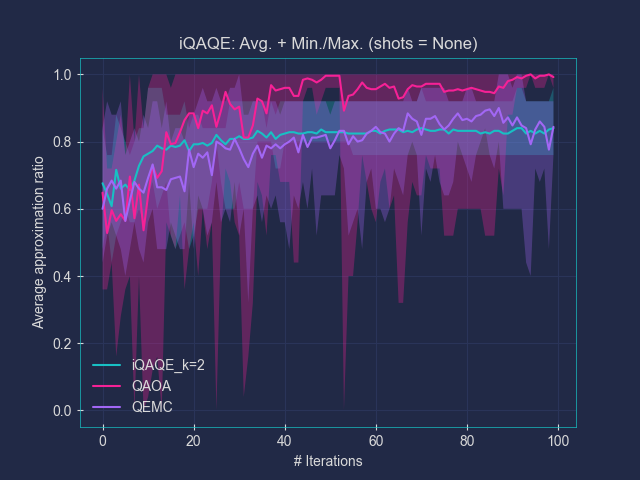
\includegraphics[width=1\textwidth]{Figures/Chapter_5/Fixed-parity/k=2(16-node).png}
      \caption{Fixed-parity \acrshort{iqaqe} for $k=2$ compared with the results from \acrshort{qaoa} and \acrshort{qemc} ($16$-node graph).}
      \label{fig:Fixed-parity/k=2(16_node)}
  \end{subfigure}
  \hfill
  \begin{subfigure}[t]{0.495\textwidth}
      \centering
      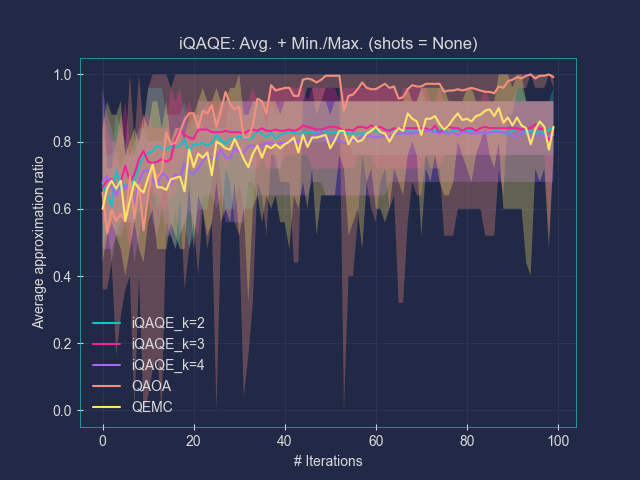
\includegraphics[width=1\textwidth]{Figures/Chapter_5/Fixed-parity/k=2_3_4(16-node).png}
      \caption{Fixed-parity \acrshort{iqaqe} for $k=2, 3$, and $4$ compared with the results from \acrshort{qaoa} and \acrshort{qemc} ($16$-node graph).}
      \label{fig:Fixed-parity/k=2,3,4(16_node)}
  \end{subfigure}
\end{figure*}

\clearpage

\begin{figure*}[ht!]
  \addtocounter{figure}{-1} % Added <<
  \centering
  \begin{subfigure}[b]{\textwidth}
      \addtocounter{subfigure}{2} % Added <<
      \centering
      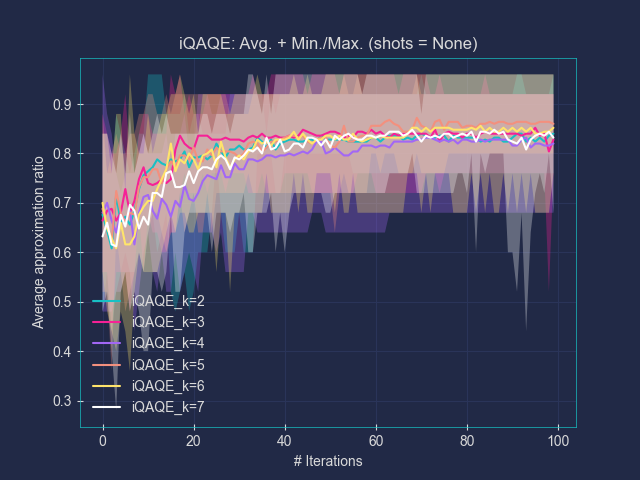
\includegraphics[width=1\textwidth]{Figures/Chapter_5/Fixed-parity/All_k's(16-node).png}
      \caption{Fixed-parity \acrshort{iqaqe} for all values of $k = 2, 3, 4, 5, 6$, and $7$ ($16$-node graph).}
      \label{fig:All_k's(16_node)}
  \end{subfigure}
  \caption{Fixed-parity polynomial-type compression scheme: numerical simulations for a $16$-node graph.}
  \label{fig:Fixed-parity(16_node)}
\end{figure*}

The previously identified trends are also apparent here. However, the performance now seems insufficient to achieve the MaxCut partition (determined by brute-force), as illustrated by the shaded areas in Figure \ref{fig:All_k's(16_node)}: the average \acrshort{ar} never quite reaches $1$. Moreover, for this graph, varying the value of $k$ does not significantly impact performance. Hence, it is advisable to choose the value of $k$ that requires the fewest qubits. In this instance, $k=3$ is optimal, needing only \texttt{n\_qubits = 6}, since $\binom{6}{3} = 20 \geq 16$.

%%%%%%%%%%%%%%%%%%%%%%%%%%%%%%%%%%%%%%%%%%%%%%%%%%%%%%%%%%%%%%%%%%%%%%%%
% \section{Other Exploratory Ideas}
% \label{section:Exploratory_Ideas}

% Other exploratory ideas and their results.

% % Send this to Chapter 6, instead.




%%%%%%%%%%%%%%%%%%%%%%%%%%%%%%%%%%%%%%%%%%%%%%%%%%%%%%%%%%%%%%%%%%%%%%%%
% \subsection{Tranche-based Oracle colouring}
% \label{section:Oracle_colouring}

% Tranche-based Oracle colouring schemes and their results.

% % Send this to Chapter 6, instead.




%%%%%%%%%%%%%%%%%%%%%%%%%%%%%%%%%%%%%%%%%%%%%%%%%%%%%%%%%%%%%%%%%%%%%%%%
\section{Extended-QEMC}
\label{section:Extended_QEMC}

Extended-QEMC scheme and variations thereof, and their results.





%%%%%%%%%%%%%%%%%%%%%%%%%%%%%%%%%%%%%%%%%%%%%%%%%%%%%%%%%%%%%%%%%%%%%%%%
\subsection{Unmodified Extended-QEMC}
\label{subsection:Vanilla_Extended_QEMC}

Vanilla Extended-QEMC scheme and variations thereof, and their results.





%%%%%%%%%%%%%%%%%%%%%%%%%%%%%%%%%%%%%%%%%%%%%%%%%%%%%%%%%%%%%%%%%%%%%%%%
\protect\subsection{Cardinality \texorpdfstring{$= k$}{= k} Extended-QEMC}
\label{subsection:Card._eq_k_Extended_QEMC}

Cardinality $= k$ Extended-QEMC scheme and variations thereof, and their results.




%%%%%%%%%%%%%%%%%%%%%%%%%%%%%%%%%%%%%%%%%%%%%%%%%%%%%%%%%%%%%%%%%%%%%%%%
\section{Alternative Ansätze}
\label{section:Alternative_ansätze}

Alternative Ansätze and their results: More specifically, Non-deterministic CNOTs. Could also feature some discussion on problem-inspired \textit{vs.} problem-agnostic Ansätze. Mention how we've been using problem-agnostic Ansätze, in iQAQE, and how this hinders the results. Explain how/why problem-inspired is better, and how we could use it in the future. (Could refer to the QML review paper, here.)




%%%%%%%%%%%%%%%%%%%%%%%%%%%%%%%%%%%%%%%%%%%%%%%%%%%%%%%%%%%%%%%%%%%%%%%%
\section{Goemans-Williamson and Bigger Graphs}
\label{section:GW_Bigger_Graphs}

Goemans-Williamson scheme and its results on bigger graphs.





%%%%%%%%%%%%%%%%%%%%%%%%%%%%%%%%%%%%%%%%%%%%%%%%%%%%%%%%%%%%%%%%%%%%%%%%
\section{Average Best-so-Far correction}
\label{section:Avg_BSF_correction}

Average Best-so-Far correction and its results. Mention how it was "wrong", initially, and how it was "fixed". I'm not sure where to include this, though.

% I think I should send these plots to an Appendix, so I can save some space.







%%%%%%%%%%%%%%%%%%%%%%%%%%%%%%%%%%%%%%%%%%%%%%%%%%%%%%%%%%%%%%%%%%%%%%%%
\section{Randomized iQAQE benchmarking}
\label{section:Randomized_iQAQE_benchmarking}

Talk about the randomized benchmarking that we've been doing, and how it's been helping us to understand the performance of the different schemes. Type $1$ and $2$ variables, etc. This could have many subsections.

% % ----------------------------------------------------------------------
% \subsection{Figures}
% \label{subsection:figures}

% Insert your section material and possibly a few figures.

% Make sure all figures presented are referenced in the text!

% The caption should appear below the figure.


% % ----------------------------------------------------------------------
% \subsubsection{Images}
% \label{subsection:images}

% By default, this document supports file types {\it .png,.pdf,.jpg,,.jpeg}.

% See the documentation of package {\it graphicx} \url{https://www.ctan.org/tex-archive/macros/latex/required/graphics/} for other extensions support.

% When referencing a figure, use the abbreviation Fig., unless it is the beginning of a sentence.

% Figure~\ref{fig:airbus1} is an example and so is Fig.~\ref{fig:aircraft}.

% \begin{figure}[!htb]
%   \centering
%   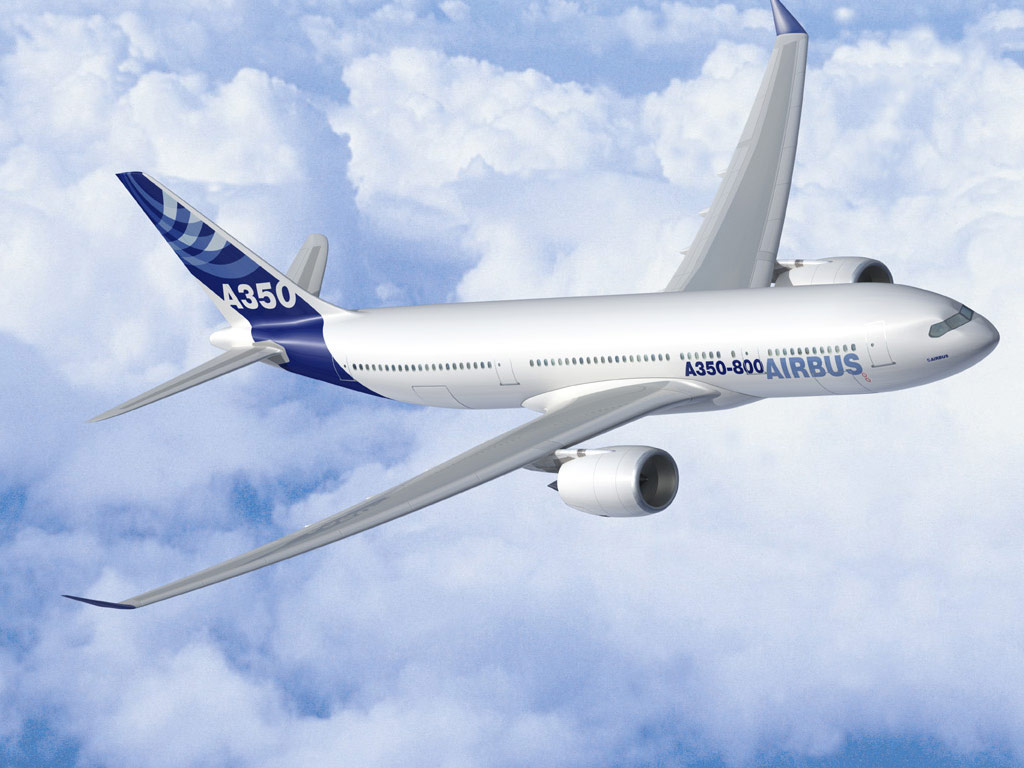
\includegraphics[width=0.25\textwidth]{Figures/Airbus_A350.jpg}
%   \caption[Optional caption for figure in TOC.]{Caption for figure.}
%   \label{fig:airbus1}
% \end{figure}

% It is possible to include subfigures.
% Figure~\ref{fig:aircraft} is composed of three subfigures: Fig.~\ref{fig:aircraft1}, \ref{fig:aircraft2} and \ref{fig:aircraft3}.
% %
% \begin{figure}[!htbp]
%     \centering
%     \subfloat[Airbus A320.\label{fig:aircraft1}]{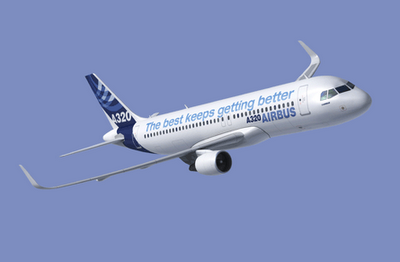
\includegraphics[width=0.49\textwidth]{Figures/Airbus_A320_sharklets.png}]{fig1a}}\hfill
%     \subfloat[Bombardier CRJ200.\label{fig:aircraft2}] {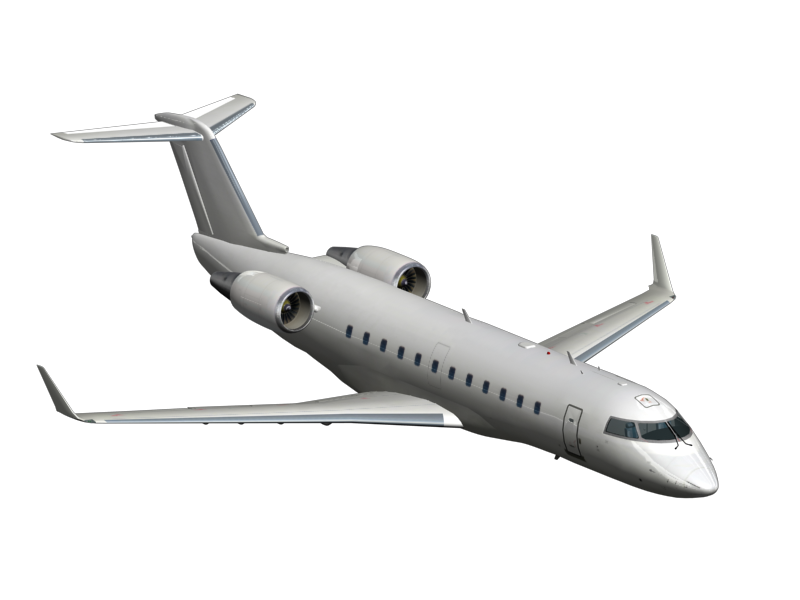
\includegraphics[width=0.49\linewidth]{Figures/Bombardier_CRJ200.png}}\hfill
%     \subfloat[Airbus A350.\label{fig:aircraft3}]{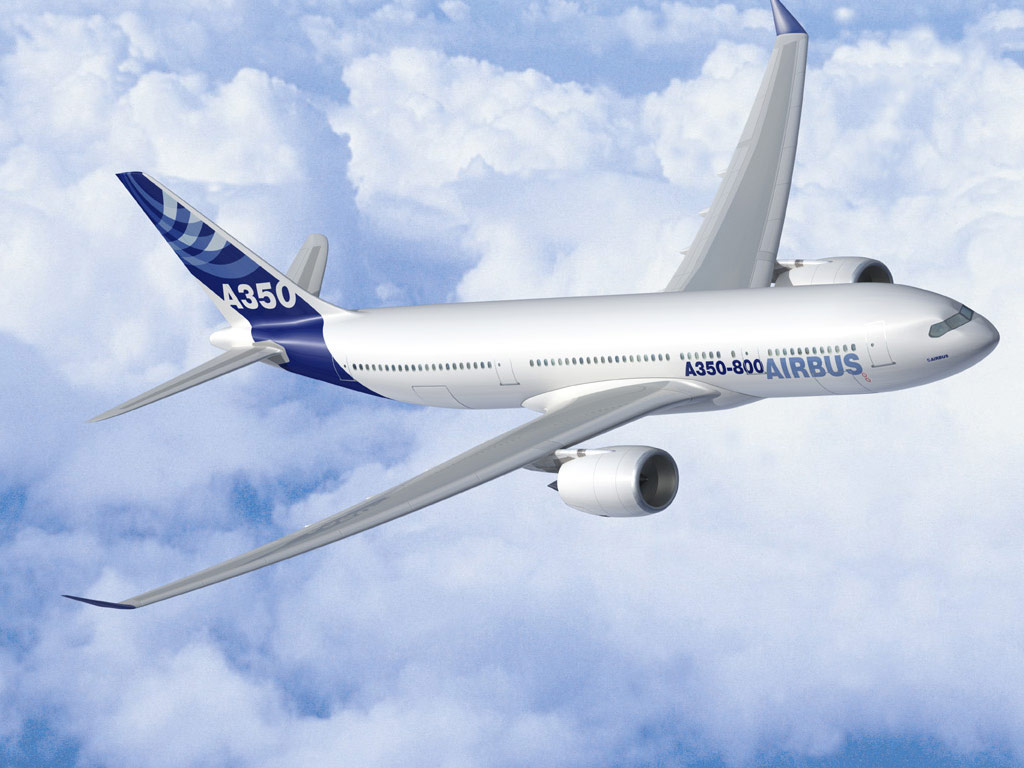
\includegraphics[width=0.49\textwidth]{Figures/Airbus_A350.jpg}}
%     \caption{Examples of aircraft.} \label{fig:aircraft}
% \end{figure}

% Most aircraft have wings with large aspect ratios (\AR = 8 -- 15) for higher aerodynamic efficiency.


% % ----------------------------------------------------------------------
% \subsubsection{Drawings}
% \label{subsection:drawings}

% Insert your subsection material and for instance a few drawings.

% The schematic illustrated in Fig.~\ref{fig:algorithm} can represent some sort of algorithm.

% \begin{figure}[!htb]
%   \centering
%   \scriptsize
% %  \footnotesize 
% %  \small
%   \setlength{\unitlength}{0.9cm}
%   \begin{picture}(8.5,6)
%     \linethickness{0.3mm}

%     \put(3,6){\vector(0,-1){1}}
%     \put(3.5,5.4){$\bf \alpha$}
%     \put(3,4.5){\oval(6,1){}}
%     %\put(0,4){\framebox(6,1){}}
%     \put(0.3,4.4){Grid Generation: \quad ${\bf x} = {\bf x}\left({\bf \alpha}\right)$}

%     \put(3,4){\vector(0,-1){1}}
%     \put(3.5,3.4){$\bf x$}
%     \put(3,2.5){\oval(6,1){}}
%     %\put(0,2){\framebox(6,1){}}
%     \put(0.3,2.4){Flow Solver: \quad ${\cal R}\left({\bf x},{\bf q}\left({\bf x}\right)\right) = 0$}

%     \put(6.0,2.5){\vector(1,0){1}}
%     \put(6.4,3){$Y_1$}

%     \put(3,2){\vector(0,-1){1}}
%     \put(3.5,1.4){$\bf q$}
%     \put(3,0.5){\oval(6,1){}}
%     %\put(0,0){\framebox(6,1){}}
%     \put(0.3,0.4){Structural Solver: \quad ${\cal M}\left({\bf x},{\bf q}\left({\bf x}\right)\right) = 0$}

%     \put(6.0,0.5){\vector(1,0){1}}
%     \put(6.4,1){$Y_2$}

%     %\put(7.8,2.5){\oval(1.6,5){}}
%     \put(7.0,0){\framebox(1.6,5){}}
%     \put(7.1,2.5){Optimizer}
%     \put(7.8,5){\line(0,1){1}}
%     \put(7.8,6){\line(-1,0){4.8}}
%   \end{picture}
%   \caption{Schematic of some algorithm.}
%   \label{fig:algorithm}
% \end{figure}


% % ----------------------------------------------------------------------
% \subsection{Equations}
% \label{subsection:equations}

% Equations can be inserted in different ways.

% The simplest way is in a separate line as

% \begin{equation}
%   \frac{{\rm d} q_{ijk}}{{\rm d} t} + {\cal R}_{ijk}({\bm q}) = 0 \,,
% \label{eq:ode}
% \end{equation}
% %
% where each variable must properly defined.

% If the equation is to be embedded in the text, it can be done like ${\partial {\cal R}}/{\partial {\bm q}}=0$.

% It may also be split in different lines like

% \begin{eqnarray}
%   {\rm Minimize}   && Y({\bm \alpha},{\bm q}({\bm \alpha}))            \nonumber           \\
%   {\rm with~respect~to}     && {\bm \alpha}                                     \label{eq:minimize} \\
%   {\rm subject~to} && {\cal R}({\bm \alpha},{\bm q}({\bm \alpha})) = 0 \nonumber           \\
%                    &&       C ({\bm \alpha},{\bm q}({\bm \alpha})) = 0 \,. \nonumber
% \end{eqnarray}

% It is also possible to use subequations.

% \begin{subequations}
%     \begin{equation}
%     \frac{\partial \rho}{\partial t} + \frac{\partial}{\partial x_j}\left( \rho u_j \right) = 0 \,,
%     \label{eq:continuity}
%     \end{equation}
%     \begin{equation}
%     \frac{\partial}{\partial t}\left( \rho u_i \right) + \frac{\partial}{\partial x_j} \left( \rho u_i u_j + p \delta_{ij} - \tau_{ji} \right) = 0, \quad i=1,2,3 \,,
%     \label{eq:momentum}
%     \end{equation}
%     \begin{equation}
%         \frac{\partial}{\partial t}\left( \rho E \right) + \frac{\partial}{\partial x_j} \left( \rho E u_j + p u_j - u_i \tau_{ij} + q_j \right) = 0 \,.
%     \label{eq:energy}
%     \end{equation}
% \label{eq:NavierStokes}%
% \end{subequations}

% Notice that the equations should be punctuated as they are part of sentences, so a comma or a period should be put at the end of each of them, as exemplified in all the previous equations.

% When referencing an equation, use the abbreviation Eq., unless it is the beginning of a sentence.
% The number of the equation should always be in parenthesis.

% Equations~(\ref{eq:continuity}), (\ref{eq:momentum}) and (\ref{eq:energy}) form the Navier--Stokes equations~(Eq.~ (\ref{eq:NavierStokes})).


% % ----------------------------------------------------------------------
% \subsection{Tables}
% \label{section:tables}

% Insert your subsection material and for instance a few tables.

% Make sure all tables presented are referenced in the text!

% The caption should appear above the table.

% Follow some guidelines when making tables:

% \begin{itemize}
%   \item Avoid vertical lines;
%   \item Avoid “boxing up” cells, usually 3 horizontal lines are enough: above, below, and after heading;
%   \item Avoid double horizontal lines;
%   \item Add enough space between rows.
% \end{itemize}

% \begin{table}[!htb]
%   \caption[Table caption shown in TOC.]{Table caption.}
%   \label{tab:aeroCoeff}
%   \renewcommand{\arraystretch}{1.2} % more space between rows
%   \centering
%   \begin{tabular}{lccc}
%     \toprule
%     Model           & $C_L$ & $C_D$ & $C_{M y}$ \\
%     \midrule
%     Euler           & 0.083 & 0.021 & -0.110    \\
%     Navier--Stokes  & 0.078 & 0.023 & -0.101    \\
%     \bottomrule
%   \end{tabular}
% \end{table}

% When referencing a table, use the abbreviation Tab., unless it is the beginning of a sentence.

% Tables~\ref{tab:memory} and \ref{tab:multipleColumns} are examples of tables with merging columns:

% \begin{table}[!htb]
%   \caption{Memory usage comparison (in MB).}
%   \label{tab:memory}
%   \renewcommand{\arraystretch}{1.2} % more space between rows
%   \centering
%   \begin{tabular}[]{lrr}
%     \toprule
%                 & \multicolumn{2}{c}{\underline{Virtual memory [MB]}} \\
%                 & Euler       & Navier--Stokes \\
%     \midrule
%       Wing only &  1,000      &    2,000       \\
%       Aircraft  &  5,000      &   10,000       \\
%       (ratio)   & $5.0\times$ & $5.0\times$    \\
%     \bottomrule
%   \end{tabular}
% \end{table}

% \begin{table}[!htb]
%   \caption{Another table caption.}
%   \label{tab:multipleColumns}
%   \centering
%   \renewcommand{\arraystretch}{1.2} % more space between rows
%   \begin{tabular}{@{}rrrrcrrr@{}} % remove space to the vertical edges @{}...@{}
%     \toprule
%       & \multicolumn{3}{c}{$w = 2$} & \phantom{abc} & \multicolumn{3}{c}{$w = 4$} \\
%     \cmidrule{2-4}
%     \cmidrule{6-8}
%       & $t=0$ & $t=1$ & $t=2$ && $t=0$ & $t=1$ & $t=2$ \\
%     \midrule
%       $dir=1$
%       \\
%       $c$ &  0.07 &  0.16 &  0.29 &&  0.36 &  0.71 &   3.18 \\
%       $c$ & -0.86 & 50.04 &  5.93 && -9.07 & 29.09 &  46.21 \\
%       $c$ & 14.27 &-50.96 &-14.27 && 12.22 &-63.54 &-381.09 \\
%       $dir=0$
%       \\
%       $c$ &  0.03 &  1.24 &  0.21 &&  0.35 & -0.27 &  2.14 \\
%       $c$ &-17.90 &-37.11 &  8.85 &&-30.73 & -9.59 & -3.00 \\
%       $c$ &105.55 & 23.11 &-94.73 &&100.24 & 41.27 &-25.73 \\
%     \bottomrule
%   \end{tabular}
% \end{table}

% An example with merging rows can be seen in Tab.~\ref{tab:multipleRows}.

% \begin{table}[!htb]
%   \caption{Yet another table caption.}
%   \label{tab:multipleRows}
%   \renewcommand{\arraystretch}{1.2} % more space between rows
%   \centering
%   \begin{tabular}{ccccc}
%     \toprule
%       \multirow{2}{*}{ABC} & \multicolumn{4}{c}{header} \\
%       \cmidrule{2-5} & 1.1 & 2.2 & 3.3 & 4.4 \\
%     \midrule
%       \multirow{2}{*}{IJK} & \multicolumn{2}{c}{\multirow{2}{*}{group}} & 0.5 & 0.6 \\
%       \cmidrule{4-5}       & \multicolumn{2}{c}{}                       & 0.7 & 1.2 \\
%     \bottomrule
%   \end{tabular}
% \end{table}

% If a table has too many columns, it can be scaled to fit the text width, as in Tab.~\ref{tab:scale}.
% %
% \begin{table}[!htb]
%   \caption{Very wide table.}
%   \label{tab:scale}%
%   \renewcommand{\arraystretch}{1.2} % more space between rows
%   \centering
%   \resizebox*{\textwidth}{!}{%
%     \begin{tabular}[]{lcccccccccc}
%       \toprule
%         Variable &  a  &  b  &  c  &  d  &  e  &  f  &  g  &  h  &  i  &  j  \\
%       \midrule
%         Test 1   &  10,000 &  20,000 &  30,000 &  40,000 &  50,000 &  60,000 &  70,000 &  80,000 &  90,000 & 100,000 \\
%         Test 2   &  20,000 &  40,000 &  60,000 &  80,000 & 100,000 & 120,000 & 140,000 & 160,000 & 180,000 & 200,000 \\
%       \bottomrule
%     \end{tabular}
%   }%
% \end{table}


% % ----------------------------------------------------------------------
% \subsection{Mixing}
% \label{section:mixing}

% If necessary, a figure and a table can be put side-by-side as in Fig.~\ref{fig:side_by_side}

% \begin{figure}[!htb]
%   \begin{minipage}[b]{0.60\linewidth}
%     \centering
%     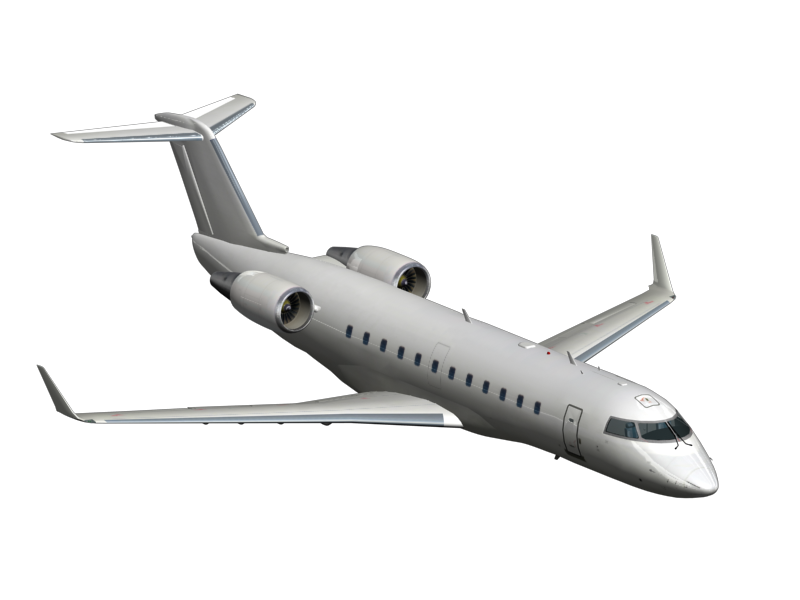
\includegraphics[width=\linewidth]{Figures/Bombardier_CRJ200}
%   \end{minipage}%
%   \begin{minipage}[b]{0.30\linewidth}
%     \centering
%     \begin{tabular}[b]{lll}
%       \toprule
%         \multicolumn{3}{c}{Legend} \\
%       \midrule
%         A & B & C \\
%         0 & 0 & 0 \\
%         0 & 1 & 0 \\
%         1 & 0 & 0 \\
%         1 & 1 & 1 \\
%       \bottomrule
%     \end{tabular}
%     \vspace{5em}
%   \end{minipage}
% \caption{Figure and table side-by-side.}
% \label{fig:side_by_side}
% \end{figure}

